\def\solenoidMotorWidth{3}
\def\solenoidMotorHeight{1.5}
\def\solenoidBoardWidth{2}
\def\solenoidBoardHeight{1}

\def\solenoidBvlX{0.3}
\def\solenoidBvlY{0.2}

\def\solenoidBoardBvlX{0.5}
\def\solenoidBoardBvlY{0.5}

\def\solenoidPinHoleThickness{0.07}

\ctikzsubcircuitdef{spicsolenoid} {
    vcc, gnd%
} {
    coordinate (#1-origin)
    ++({\solenoidMotorWidth/2},{(-\solenoidMotorHeight-\solenoidBoardHeight)/2})
    node [inner sep = 0pt, anchor = center] {
        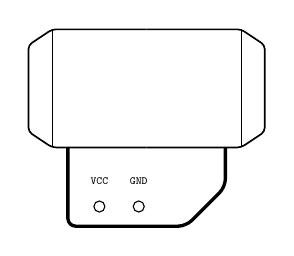
\begin{tikzpicture}
            \draw [semithick, rounded corners = 1mm]
            (0,0) coordinate (origin)
            (origin) ++({\solenoidMotorWidth/2},0)
            coordinate (mid)
            ;
            %% drawing motor
            \draw [semithick, rounded corners = 0.5mm]
            (mid) -- ++({(-\solenoidMotorWidth/2)+\solenoidBvlX},0)
            -- ++(-\solenoidBvlX,-\solenoidBvlY)
            -- ++(0,{-\solenoidMotorHeight+(2*\solenoidBvlY)})
            -- ++(\solenoidBvlX,-\solenoidBvlY)
            -- ++({(\solenoidMotorWidth/2)-\solenoidBvlX},0)
            ;
            \draw [semithick, rounded corners = 0.5mm]
            (mid) -- ++({(\solenoidMotorWidth/2)-\solenoidBvlX},0)
            -- ++(\solenoidBvlX,-\solenoidBvlY)
            -- ++(0,{-\solenoidMotorHeight+(2*\solenoidBvlY)})
            -- ++(-\solenoidBvlX,-\solenoidBvlY)
            -- ++({(-\solenoidMotorWidth/2)+\solenoidBvlX},0)
            ;
            %%
            \draw [thin]
            (origin) ++(\solenoidBvlX,0)
            -- ++(0,-\solenoidMotorHeight)
            (origin) ++({\solenoidMotorWidth-\solenoidBvlX},0)
            -- ++(0,-\solenoidMotorHeight)
            ;
            %% board
            \draw [very thick, rounded corners = 1mm]
            (mid) ++({\solenoidBoardWidth/2},-\solenoidMotorHeight)
            -- ++(0,{-\solenoidBoardHeight+\solenoidBoardBvlY})
            -- ++(-\solenoidBoardBvlX,-\solenoidBoardBvlY)
            -- ++({-\solenoidBoardWidth+\solenoidBoardBvlX},0)
            -- ++(0,\solenoidBoardHeight)
            ;
            %% inputs
            \draw
            (origin) ++(
            {(\solenoidMotorWidth-\solenoidBoardWidth)/2},
            {-\solenoidMotorHeight-\solenoidBoardHeight}
            )
            ++(0.4,0.25)
            circle (\solenoidPinHoleThickness)
            node [above = 5pt, font = \tiny, scale = 0.8] {\texttt{VCC}}
            ++(0.5,0)
            circle (\solenoidPinHoleThickness)
            node [above = 5pt, font = \tiny, scale = 0.8] {\texttt{GND}}
            ;
        \end{tikzpicture}
    }
    (#1-origin) ++(
    {(\solenoidMotorWidth-\solenoidBoardWidth)/2},
    {-\solenoidMotorHeight-\solenoidBoardHeight}
    )
    ++(0.4,0) coordinate (#1-vcc)
    ++(0.5,0) coordinate (#1-gnd)
}

\ctikzsubcircuitactivate{spicsolenoid}
